\chapter{IPv6 - Advanced Router Delegation}
\begin{itemize}
    \item In This Topology we use Router advertisement 
    \item It is stateless protocol where no information is stored about the client in the routers.
\end{itemize}
\label{IPv6 - Advanced Router Delegation}
\begin{figure}[H]
\centering
  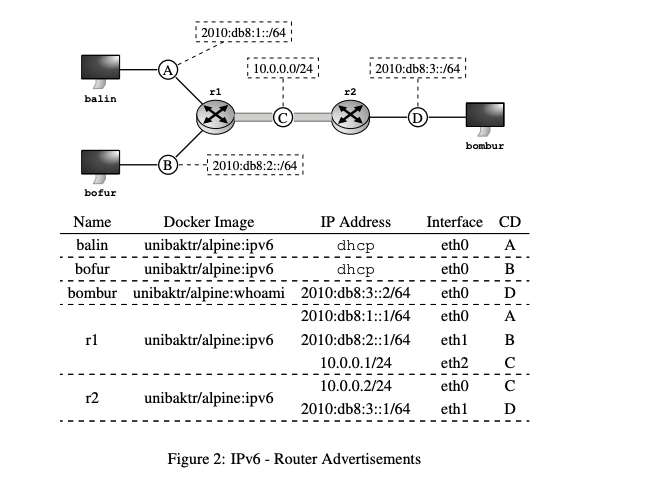
\includegraphics[width=0.9\textwidth]{images/Topology-2.png}
  \caption{Advanced Router Delegation Topology}
  \label{fig:2.1 }
  \end{figure}
  \section{Configuration on R1}
  \subsection{Managed router advertisement}
  \begin{itemize}
    \item Managed router advertisements for CD A ranging from 2010:db8:1::100/64 to 2010:db8:1::200/64.
    \item on r1 create a /etc/radvd.conf  file and add the managed router advertisement code
    \item radvd file will send route advertisements to all the nodes on
       the network.  
       \item for interface 0 router 1 advertises a range of 2010:db8:1::100/64 to 2010:db8:1::200/64 address to balin ,so that it accepts the traffic entering this range of address from balin 
    \end{itemize}
\begin{figure}[H]
\centering
  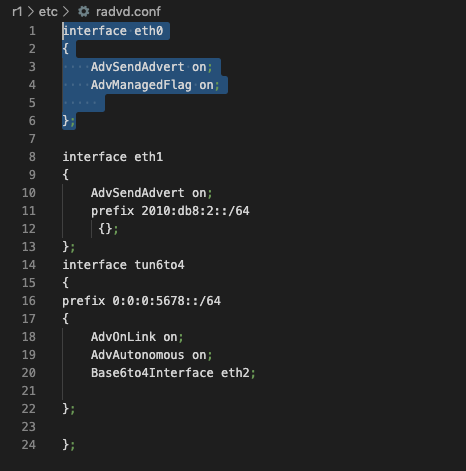
\includegraphics[width=0.9\textwidth]{images/managed advertisement.png}
  \caption{Managed Advertisement}
  \label{fig:2.2 }
  \end{figure}
  \begin{itemize}
    \item we have added the managed advertisement for interface 0 of router 1 as highlighted in the above picture
    \item AdvManagedFlag : when it is set to 'on' it uses the administered stateful protocol for address  auto configuration.By default this flag will be off.
    \end{itemize}
\subsection{Unmanaged router advertisement}
\begin{figure}[H]
\centering
  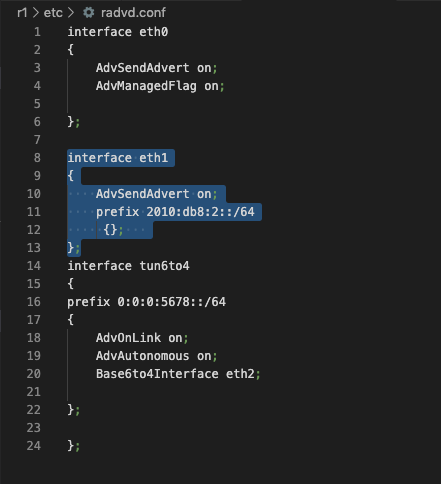
\includegraphics[width=0.9\textwidth]{images/unmanged router advertisement.png}
  \caption{Unmanaged Advertisement}
  \label{fig:2.3 }
  \end{figure}
 \begin{itemize}
\item Unmanaged router advertisements for CD B 2010:db8:2::/64
\item As highlighted in the above picture interface 1 of router 1 advertises 2010:db8:2::/64 address to bofur .
\item In this section we have used prefix:2010:db8:2::/64 which means we only advertise this address to bofur and accept the traffic flowing through this address from bofur.
\end{itemize}

\section{6-to-4 tunnel establishment}
\begin{itemize}
\item To establish connection between r1 and r2 we need to enable IPv6 traffic. As r1 and r2 are assigned with IPv6 addresses and CD is assigned with IPv4, we can not establish a connection between them.
\item Below screenshot shows the config/code part that helps to establish the 6-to-4 tunnelling.
\begin{figure}[H]
\centering
  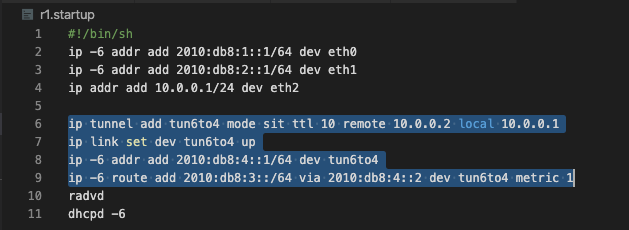
\includegraphics[width=0.9\textwidth]{images/6to4Tunnelling_r1.png}
  \caption{6-to-4 tunnelling in r1}
  \label{fig:2.4 }
\end{figure}
\begin{figure}[H]
\centering
  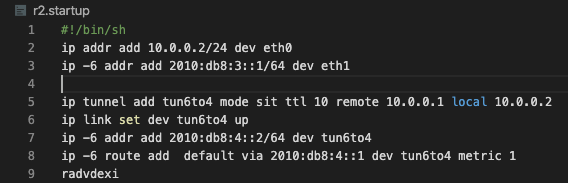
\includegraphics[width=0.9\textwidth]{images/6to4Tunnelling_r2.png}
  \caption{6-to-4 tunnelling in r2}
  \label{fig:2.5}
\end{figure}
\item A 6to4 tunnel interface automatically converts the 32 bits in its IPv6 address following this prefix to a global unicast IPv4 address for transport across an IPv4 network such as the public Internet.
\end{itemize}

\section{Checking Global connectivity}
\begin{itemize}
\item To establish global connectivity we have added assigned addresses to all the machines and provided default routers wherever required as per the given data.
\item Below screenshots shows the connectivity between the machines
\begin{figure}[H]
\centering
  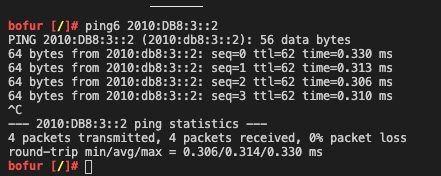
\includegraphics[width=0.9\textwidth]{images/BofurToBombur.png}
  \caption{Connectivity between bofur to bombur}
  \label{fig:2.6}
\end{figure}
\item To connect to balin we need get the IP assigned by dhcp. Using Ifconfig we can get the address assigned to balin as below,
\begin{figure}[H]
\centering
  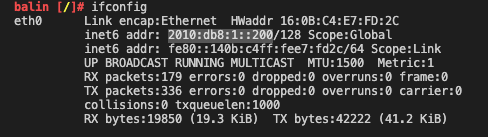
\includegraphics[width=0.9\textwidth]{images/BalinIPByDHCP.png}
  \caption{IP assigned to balin by dhcp}
  \label{fig:2.7}
\end{figure}

\begin{figure}[H]
\centering
  \includegraphics[width=0.9\textwidth]{images/BalinToBombur.png}
  \caption{Connectivity between balin to bombur}
  \label{fig:2.8}
\end{figure}
\begin{figure}[H]
\centering
  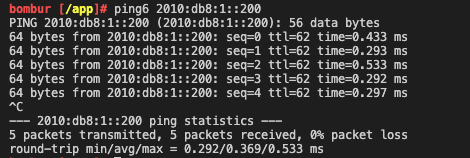
\includegraphics[width=0.9\textwidth]{images/BofurToBalin.png}
  \caption{Connectivity between bombur to balin}
  \label{fig:2.9}
\end{figure}
\end{itemize}

\section{Wireshark and 6-to-4 tunnel functionalities}
\begin{itemize}
\item We can not capture the curl with wireshark in windows and Mac systems.
\subsection{6-to-4 functionalities}
\item It enables encapsulation of IPv6 packets into IPv4 for transport across an IPv4 network.
\item It allows for automatic IPv6-to-IPv4 address translation, and treats the underlying IPv4 network as one big non-broadcast multiaccess (NBMA) network, rather than a collection of independent point-to-point links.
\end{itemize}
